

\part{An\'alisis de datos de microarrays}

\chapter{El proceso de an\'alisis de datos de microarray (MDA)\label{MDAProcess}}

\section{Introducci\'on}

Este cap\'itulo es una corta transici\'on entre la primera parte del curso, en la que se han presentado los conceptos y herramientas b\'asicos y la segunda en donde se presentan por separado y con mayor detalle los m\'etodos de an\'alisis de datos de microarrays.

Su objetivo por tanto es ofrecer una visi\'on \emph{de conjunto} que sirva de gu\'ia (``roadmap'') para los cap\'itulos siguientes de forma que sin perder el detalle de cada uno de ellos tengamos conciencia de en que punto del proceso general nos encontramos.

El cap\'itulo se estructura en dos partes. En la primera se presentan brevemente algunos de los problemas que t\'ipicamente se puede querer estudiar con microarrays u otras t\'ecnicas similares de an\'alisis de datos de alto rendimiento. A continuaci\'on se presenta lo que se ha llamdo aqu\'i el \emph{proceso de an\'alisis de microarrays}. Finalmente se intoducen algunos casos reales que, a modo de ejemplo se utilizar\'an en los cap\'itulos siguientes.

\section{Tipos de estudios}

Los microarrays y otras tecnolog\'ias de alto rendimiento se han aplicado a multitud de investigaciones, de tipus muy diversos que van desde estudio del cancer  (\cite{alizadeh:2000, Golub:1999, vantveer:2002}) al de la germinaci\'on y la maduraci\'on del tomate (\cite{Moore:2002}). A pesar de ello no resulta complicado clasificar los estudios realizados en algunos de los grandes bloques que se describen a continuaci\'on. La clasificaci\'on est\'a basada en el excelente texto de Simon y colegas (\cite{Simon:2003}) y aunque se origina en problemas de microarrays se puede aplicar f\'acilmente a estudios de gen\'omica o ultrasecuenciaci\'on.

\subsection{Comparaci\'on de grupos o \emph{Class comparison}}

El objetivo de los estudios comparativos es determinar si los perfiles de expresi\'on g\'enica difieren entre grupos previamente identificados. Tambi\'en se conoce estos estudios como de \emph{selecci\'on de  genes diferencialmente expresados} y son, sin duda los m\'as habituales. Los grupos pueden representar una gran variedad de condiciones, desde distintos tejidos a distintos tratamientos o m\'ultiples combinaciones de factores experimentales.

El an\'alisis de este tipo de experimentos, que se describe en el cap\'itulo sobre selecci\'on de genes diferencialmente expresados utiliza herramientas estad\'isticas como las pruebas de comparaci\'on de grupos param\'etricas (t de Student) o no (test de Mann-Whitney) o diversos m\'etodos de an\'alisis de la varianza.

Entre los ejemplos de la secci\'on ~\ref{c4examples} los casos  ~\ref{celltypes}, ~\ref{estrogen} o ~\ref{CCL4} hacen referencia a estudios comparativos.

\subsection{Predicci\'on de clase o \emph{Class prediction}}

La predicci\'on de clase puede confundirse con la selecci\'on de genes en tanto que disponemos de clases predefinidas pero su objetivo es distinto, ya que no pretende simplemente buscar genes cuya expresi\'on sea distinta entre dichos grupos sino genes que puedan ser utilizados para identificar a que clase pertenece un ``nuevo'' individuo dado cuya clase es ``a priori'' desconocida. El proceso de predicci\'on suele empezar con una selecci\'on de genes informativos, que pueden ser, o no, los mismos que se obtendr\'ian si aplic\'aramos los m\'etodos del apartado anterior, seguida de la construcci\'on de un modelo de predicci\'on y, lo que es m\'as importante, de la verificaci\'on o validaci\'on de dicho modelo con unos datos nuevos independientes de los utilizados para el desarrollo del modelo.

Aunque el inter\'es de la predicci\'on de clase es muy alto se trata de un procedimiento mucho m\'as complejo y con m\'as posibilidades de error que la simple selecci\'on de genes diferencialmente expresados.

Entre los ejemplos de la secci\'on ~\ref{c4examples} el caso  ~\ref{golub} trata de un problema de predicci\'on, a la vez que uno de descubrimiento de clases.

\subsection{Descubrimiento de clases o \emph{Class discovery}}

Un problema distinto a los descritos se presenta cuando no se conoce las clases en que se agrupan los individuos. En este caso de lo que se trata es de encontrar grupos entre los datos que permitan reunir a los individuos m\'as parecidos entre si y distintos de los de los dem\'as grupos. Los m\'etodos estad\'isticos que se emplearan en estos casos se conocen como \emph{an\'alisis de clusters} y no son tan complejos como los de predicci\'on de clase aunque algunos aspectos como por ejemplo la definici\'on del n\'umero de grupos no resulta tampoco sencillo.

Entre los ejemplos de la secci\'on \ref{c4examples} tanto el caso \texttt{golub}, en parte, como el ~\ref{breastTum}  tratan problemas de descubrimiento de clases.

Una curiosidad del campo de la estad\'istica es que el t\'ermino clasificaci\'on aparece usado de forma indistinta para referirse a problemas de predicic\'on de clase o de descubrimiento de clase.

\subsection{Otros tipos de estudios}

Una vez identificados los principales tipos de estudios quedan muchos que no coinciden plenamente con ninguno de ellos. Sin entrar en detalles podemos se\~nalar los estudios de evoluci\'on a lo largo del tiempo  (``time course''), los de significaci\'on biol\'ogica (``Gene Enrichment Analysis'', ``Gene Set Enrichment Analysis'', ...) , los que buscan relaciones entre los genes (``network analysis'' o ``pathway analysis''). De momento con conocer e identificar los tres grandes bloques mencionados resultar\'a m\'as que suficiente.


\section{Algunos ejemplos concretos \label{c4examples}}

Una de las dificultades con que se encuentra la persona que comienza en el an\'alisis de datos de microarrays es de donde obtener ejemplos concretos con los que pr\'acticar las t\'ecnicas que est\'a aprendiendo.

No es dif\'icil encontrar datos de microarrays en internet por lo que
se han seleccionado algunos conjuntos de datos interesantes para
utilizarlos de ejemplo a lo largo del curso. Algunos de \'estos son
``populares'' en el sentido de que han sido utilizados en diversas
ocasiones y por lo tanto se encuentran bien documentados. Otros se han
escogido simplemente porque ilustran bien algunas de las ideas que se
desea exponer o por su accesibilidad.

Todos los datos corresponden a investigaciones publicadas por lo que no se describen exhaustivamente sin\'o que se expone brevemente el origen y objetivos del trabajo --incluyendo su clasificaci\'on seg\'un los grupos definidos en la secci\'on anterior-- y las caracter\'isticas perinentes para el an\'alisis como el tipo de microarrays, los grupos --si los hay-- o como acceder a los datos.

\subsection{Estudio de procesos regulados por citoquinas \label{celltypes}}
\underline{Efecto de la estimulaci\'on con LPS sobre los procesos regulados por citoquinas }

Este conjunto de datos, que se denominar\'a ``celltypes'', corresponde a un estudio realizado por Chelvarajan y sus colegas (\cite{Chelvarajan:2006}) que analizaron el efecto de la estimulaci\'on con lipopolisac\'aridos en la regulaci\'on por parte de citoquinas de ciertos procesos biol\'ogicos relacionados con la inflamaci\'on.

Este estudio es del tipo ``class comparison'' es decir su principal objetivo es la obtenci\'on de genes diferencialmente expresados entre dos o m\'as condiciones.

Los datos se encuentran disponibles en la base de datos p\'ublica \texttt{caarray} mantenida por el \emph{National Institute of Health (NIH)}, pero pueden descargarse de la p\'agina de materiales del curso para garantizar su disponibilidad.

\subsection{Clasificaci\'on molecular de la leucemia\label{golub}}

\underline{Clasificaci\'on molecular para distinguir variantes de leucemia mielobl\'astica aguda }

A finales de los a\~nos 90, Todd Golub y sus colaboradores (\cite{Golub:1999}) realizaron uno de los estudios m\'as populares hasta el momento con datos de microarrays. En \'el utilizaron microarrays de oligonucle\'otidos para 6817 genes humanos para mirar de encontrar una forma de distinguir (clasificar) tumores de pacientes con leucemia linfobl\'astica aguda (ALL) de aquellos que sufr\'ian de leucemia mieloide aguda (AML).
Adem\'as se interesaba por la posibilidad de descubrir subgrupos de forma que pudieran definirse variantes de cada una de estas patolog\'ias a nivel molecular.

La diversidad de objetivos del estudio lleva a clasificarlo tanto entre los del tipo de predicci\'on de clase como entre los que buscan descubrir nuievas clases o grupos en los datos.

Los datos de este estudio se encuentran disponibles en la web del instituto Broad, en donde se llev\'o a cabo (\href{http://www.broadinstitute.org}{http://www.broadinstitute.org}). Tambi\'en se encuentra disponible un paquete de \texttt{R} denominado \texttt{ALL} que permite utilizarlos directamente usando \texttt{R} y Bioconductor.

\subsection{Efecto del estrogeno y el tiempo de administraci\'on\label{estrogen}}

\underline{Efecto del tratamiento con estr\'ogenos en la expresi\'on de genes relacionados con c\'ancer de mama }

Scholtens y colegas (\cite{Scholtens:2004}) describen un estudio sobre el efecto de un tratamiento con estr\'ogenos y del tiempo transcurrido desde el tratamiento en la expresi\'on g\'enica en pacientes de c\'ancer de mama. Los investigadores supusieron que los genes asociados con una respuesta temprana podr\'ian considerarse dianas directas del tratamiento,
mientras que los que tardaron m\'as en hacerlo podr\'ian considerarse objetivos secundarios correspondientes a dianas m\'as alejadas en las
v\'ias metab\'olicas.

Estos datos han sido utilizados multitud de veces en los cursos de an\'alisis de microarrays realizados por el proyecto Bioconductor y se encuentran disponibles en forma de paquete de \texttt{R}, el paquete \texttt{estrogen}. Una cracater\'istica importante de este paquetes es el hecho de que en vez de los datos procesados proporciona  los datos ``crudos''en forma de archivos .CEL de Affymetrix. Esto permite una mayor flexibilidad a la hora de reutilizarlos lo que explica su popularidad.

\subsection{Efecto del CCL4 en la expresi\'on g\'enica\label{CCL4}}

\underline{Efecto del tratamiento con dimetilsulf\'oxido (DMSO) en la expresi\'on g\'enica }

Holger y colegas de la empresa LGC Ltd. en Teddington, Inglaterra realizaron unos expeimentos con microarrays de dos colores en los que trataron hepatocitos de rat\'on con tetraclorido de carbono (CCL4) o con dimetilsulf\'oxido (DMSO). El tetraclorido de carbono fue ampliamente utilizado en productos de limpieza o refrigeraci\'on para el hogar hasta que se detect\'o que pod\'ia tener efectos t\'oxicos e incluso cancer\'igenos. El DMSO es un solvente similar, sin efectos t\'oxicos conocidos, que se utiliz\'o como control negativo.

Los datos de este estudio no han sido publicados pero se encuentran disponibles en el paquete \texttt{CCL4} de bioconductor. Su inter\'es reside por un lado en que se trata de datos de microarrays de dos colores de la marca Agilent --en un momento en que la mayor\'ia de estudios se realizan con datos de un color. Aparte de esto cabe resaltar el hecho de que el paquete incluye, de forma similar al anterior, los datos ``crudos'' en forma de archivos de tipo ``Genepix'' uno de los programas populares para escanear im\'agenes generadas con microarrays de dos colores.

Este estudio es tambi\'en un estudio de comparaci\'on de clases cuyo objetivo principal es la selecci\'on de genes cuya expresi\'on se asocia al tratamiento con CCL4 o DMSO.


\subsection{An\'alisis de patrones en el ciclo celular\label{yeast}}

\underline{Busqueda de patrones de coexpresi\'on en datos de ciclo celular de levadura
}
Los datos de este ejemplo denominado \texttt{kidney} son datos ya normalizados referidos a la expresi\'on de los genes en distintos momentos del ciclo delular de la levadura e decir desde que concluye la divisi\'on celular hasta que se inicia la siguiente.

Los datos puede desargarse desde la p\'agina del proyecto ``Yeast Cell Cycle Project'' (Proyecto de estudio del ciclo celular de la levadura) en la direcci\'on:\\
\href{http://genome-www.stanford.edu/cellcycle/data/rawdata/}{http://genome-www.stanford.edu/cellcycle/data/rawdata/}.


\subsection{Recapitulaci\'on}

La tabla \ref{ejemplosEstudios} resume la lista de ejemplos que se utilizan en este manual indicando el nombre con que nos referiremos de aqu\'i en adelante a cada conjunto de datos as\' como algunas de sus carcater\'isticas.

\begin{table}[!h]
\titoltaula[0cm]{Tabla \ref{ejemplosEstudios}. Conjuntos de datos utilizados en este manual. Aparte del nombre (arbitrario y ``mnemot\'ecnico'') se indica el tipo de microarrays, el n\'umero de muestras, y el tipo de problema para el que se utilizaron originalmente.}
\begin{tabular}{|l|c|c|c|}
\hline
Nombre & Tipo & N. Muestras & Tipo de estudio  \\ \hline
\texttt{celltypes} & Un color (Affy, Mouse 4302) & 12 & Comparativo \\ \hline
\texttt{golub}     & Un color (Affy, HGU95A)  & 38  & Clasificaci\'on \\ \hline
\texttt{estrogen}  & Un color (Affy, HGU95A)  & 8 & Comparativo \\ \hline
\texttt{CCL4}     & Dos colores (Agilent, WG Rat Microarray)    & 16 & Comparativo \\ \hline
\texttt{breastTum} & Un color  (Affy, HGU95A) & 49 & Clasificaci\'on \\ \hline
\end{tabular}
\label{ejemplosEstudios}
\end{table}


\section{El proceso de an\'alisis de microarrays}

Una vez descritos los tipos de an\'alisis y algunos ejemplos podemos pasar a describir el proceso de an\'alisis de microarrays que se resume brevemente en la figura ~\ref{c04analysisProcess}.

El an\'alisis de microarrays, como la mayor\'ia de an\'alisis debe proceder de forma ordenada y siguiendo el m\'etodo cient\'ifico:
\begin{itemize}
\item La pregunta y su contexto nos servir\'an de gu\'ia para definir el \emph{Dise\~no experimental} adecuado.
\item El experimento se deber\'a realizar siguiendo las pautas decididas en el \emph{Dise\~no experimental} y los datos obtenidos
--que solemos denominar datos ``crudos'' o ``raw data''-- deber\'an someterse a los \emph{Controles de calidad adecuados} antes de continuar con su an\'alisis.
\item Una vez decidido si la calidad de los datos es aceptable pasaremos a prepararlos para el an\'alisis lo que puede incluir diversas formas
de \emph{preprocesado, o transformaciones} que a menudo se incluyen de forma general bajo el paraguas del t\'ermino \emph{normalizaci\'on}, aunque, como veremos se trata de conceptos distintos.
\item Los datos normalizados se utilizar\'an para los \emph{an\'alisis estad\'isticos} que hayamos decidido realizar durante el dise\~no experimental.
\item Finalmente los resultados de los an\'alisis ser\'an la base para una \emph{interpretaci\'on biol\'ogica} de los resultados del experimento.
\end{itemize}


\textD{Figura \ref{c04analysisProcess}}{El an\'alisis de microarrays puede ser f\'acilmente visualizado como un proceso que empieza por una
pregunta biol\'ogica y concluye con una interpretaci\'on de los resultados de los an\'alisis que, de alguna forma,
confiamos nos acerque un poco a la respuesta de la pregunta inicial.}

\vspace{-0.5cm}
\begin{figure}[!h]
\titolfigura[0cm]{Figura \ref{c04analysisProcess}. Proceso de an\'alisis de microarrays}
\label{c04analysisProcess}
\fbox{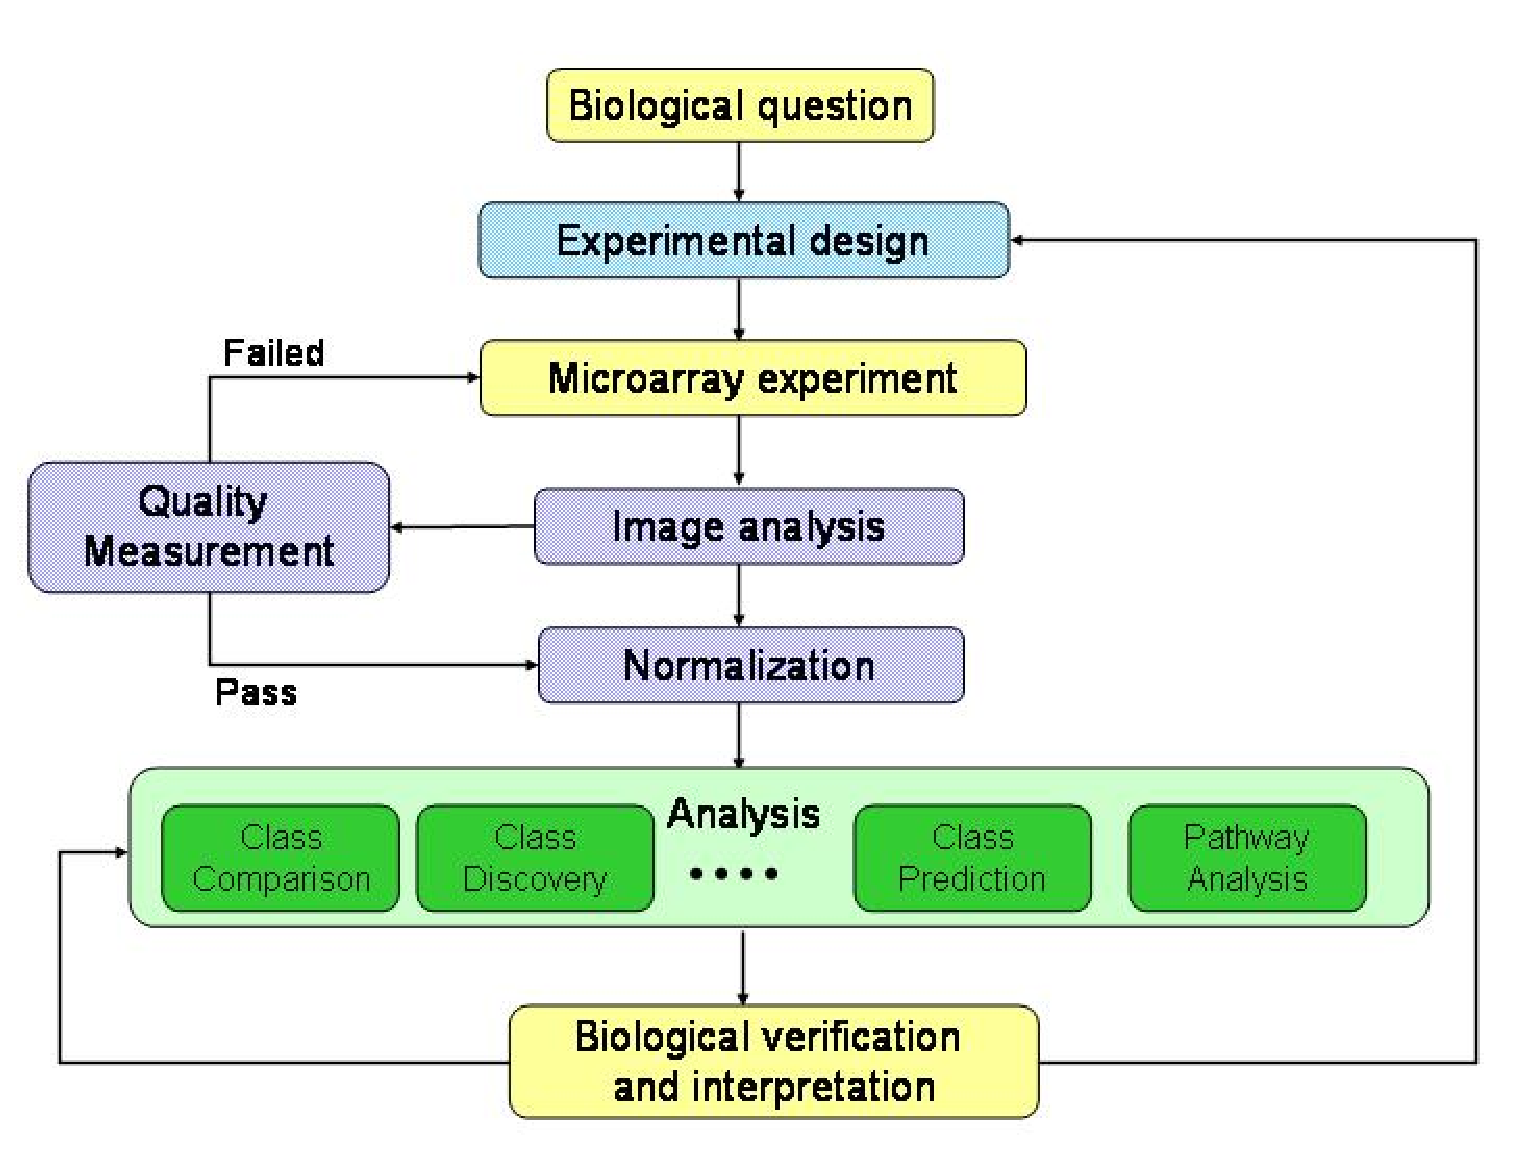
\includegraphics[height=6cm,width=0.75\textwidth]{epsimages/c04analysisProcess.eps}}
\end{figure}



El proceso descrito es b\'asicamente una forma razonable de proceder en general.
Los microarrays y otros datos gen\'omicos son diferentes en su naturaleza de
los datos cl\'asicos alrededor de los que se han desarrollado la mayor parte de
t\'ecnicas estad\'isticas. En consecuencia, en muchos casos ha sido necesario
adaptar las t\'ecnicas existentes o desarrollar otras nuevas para adecuarse a las nuevas situaciones encontradas.
Esto ha determinado que existan muchos m\'etodos para cada una de los pasos descritos anteriormente lo que da lugar a una grand\'isima cantidad de
posibilidades.

En la pr\'actica lo que suele hacerse es optar por utilizar algunos de los m\'etodos en los que hay un cierto consenso acerca de su calidad y
utilidad para cada problema. Allison (\cite{Allison:2006a}) repasa los puntos principales de este consenso dando una lista de puntos a tener en
cuenta en cualquier estudio que utilice microarrays. Imbeaud y Auffray (\cite{Imbeaud:2005}) citan una lista de hasta 39 puntos que uno debe
seguir en un experimento con microarrays para usar ``buenas pr\'acticas''.

Finalmente Zhu y otros (\cite{Zhu:2010}) utilizan un conjunto de
arrays con valores de expresi\'on conocidos para proponer los que, a su parecer, resultan los m\'etodos m\'as apropiados para cada etapa desde la
correcci\'on del backround hasta la selecci\'on de genes diferencialmente expresados.
La figura ~\ref{c04preferredAnalysisMethods} ilustra algunas de las opciones sugeridas por dichos autores.

\vspace{-0.5cm}
\begin{figure}[!h]
\titolfigura[0cm]{Figura \ref{c04preferredAnalysisMethods}. Dise\~no de arrays.}
\label{c04preferredAnalysisMethods}
\fbox{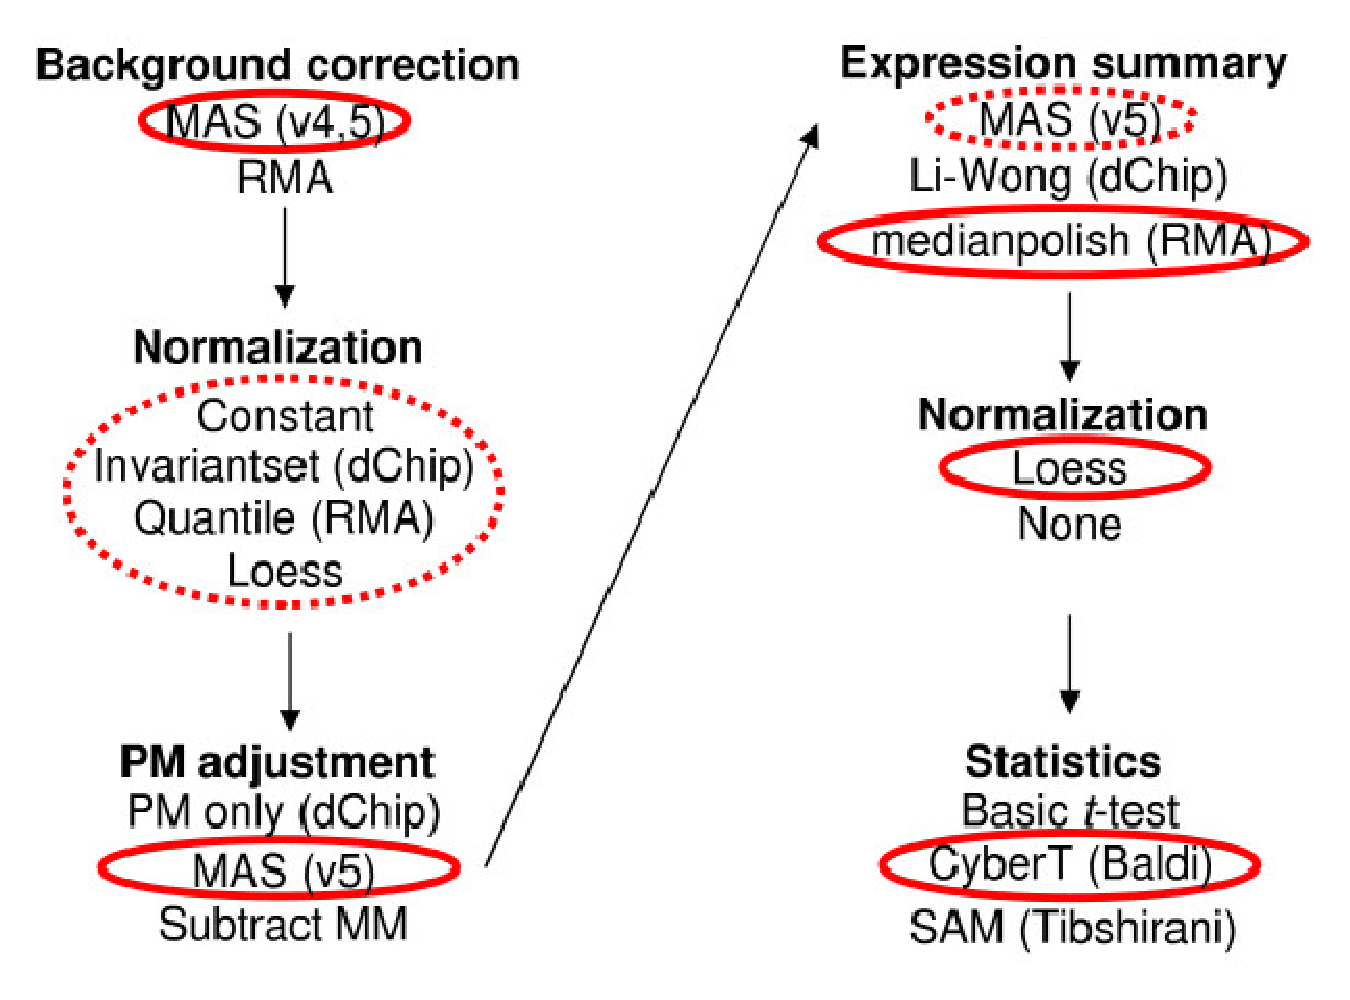
\includegraphics{epsimages/c04preferredAnalysisMethods.eps}}
\end{figure}

Los cap\'itulos que siguen al presente proceden aproximadamente en el orden del proceso descrito en ~\ref{c04preferredAnalysisMethods}.
Se empieza por tratar los principios del dise\~no de experimentos.
A continuaci\'on se describen algunos m\'etodos para el control de calidad, el preprocesado y la normalizaci\'on de los datos.
Se sigue con los m\'etodos de selecci\'on de genes --adaptados de los m\'etodos descritos en el cap\'itulo ~\ref{chapFundEst}, y los m\'etodos de
clasificaci\'on, para concluir con una introducci\'on a los m\'etodos de an\'alisis de la significaci\'on biol\'ogica de las listas de genes obtenidas
de los procesos anteriores.

